\documentclass[../main.tex]{subfiles}
\graphicspath{{\subfix{../images/}}}
\begin{document}

% \subsubsection{LiDAR–LiDAR Calibration} \label{results_lidarLidar_calib}

% Calibration was performed using the manufacturer’s Livox Viewer software, which provides real-time point cloud visualization and the ability to view, modify, and store sensor extrinsic measurements on-device.
% This interface enables manual adjustment and fine-tuning to minimize misalignment across large planar surfaces such as walls.  
% Once optimal alignment is achieved, the extrinsic parameters can be stored in each sensor’s onboard memory.
% The port and starboard Livox units use this information to transform the data into the central Livox frame prior to transmission, reducing the computational load on Atlas. 

Calibration was performed using the Livox Viewer software, which provides real-time multi-sensor point cloud visualization and tools for automatic calibration and manual adjustment of extrinsic parameters (as shown in Figure~\ref{fig:LidarLidar_calib}). 
The calibration process involved fine-tuning of the $x, y, z$ distance and roll, pitch, and yaw between sensors.
% until a consistent alignment was achieved across overlapping fields of view, using the large planar surfaces of the laboratory walls as a reference. 
Calibration accuracy was then verified through visual inspection of large, well-defined environmental features such as trees and buildings at distances of 100–200~m, confirming consistent alignment across all three sensors.
Once satisfactory alignment was reached, the resulting parameters were recorded and written to the respective sensor’s onboard memory, where the transformation can be applied before data transmission, thus minimizing downstream computation. 

% \begin{figure}[ht]
% \centering
%         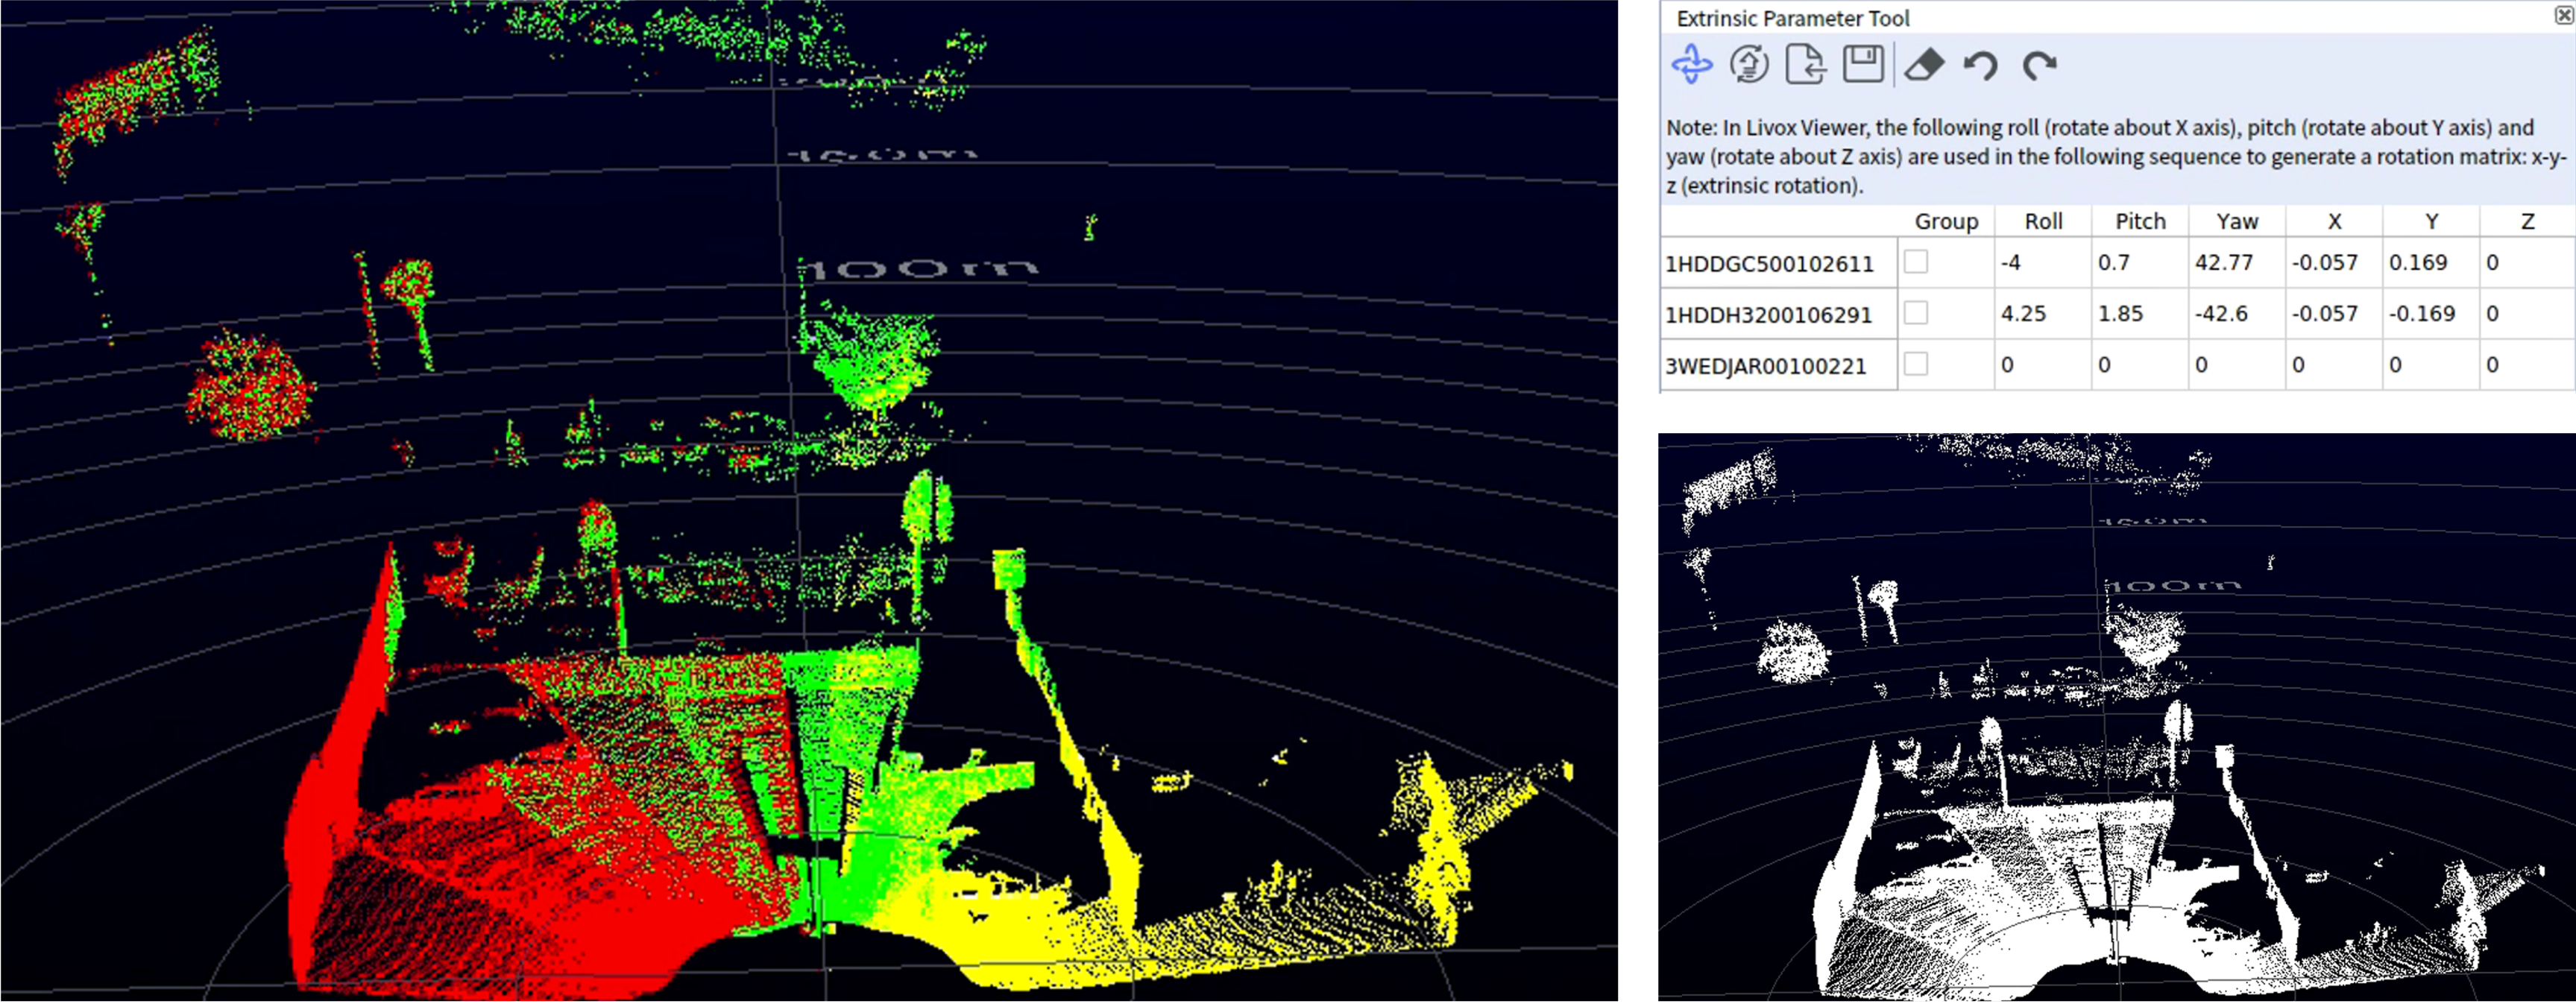
\includegraphics[width=0.95\textwidth]{Images/livox_viewer.png} 
% \caption{Data from port (red), center (green), and starboard (yellow) Livox Units as viewed within the Livox Viewer software (left), and the integrated calibration tool with estimated extrinsic parameters shown (right). }
% \label{fig:LidarLidar_calib}
% \end{figure}

\end{document}